\begin{tabular}{c c}
    \subfloat[0\%]{
      \resizebox{.45\textwidth}{!}{
      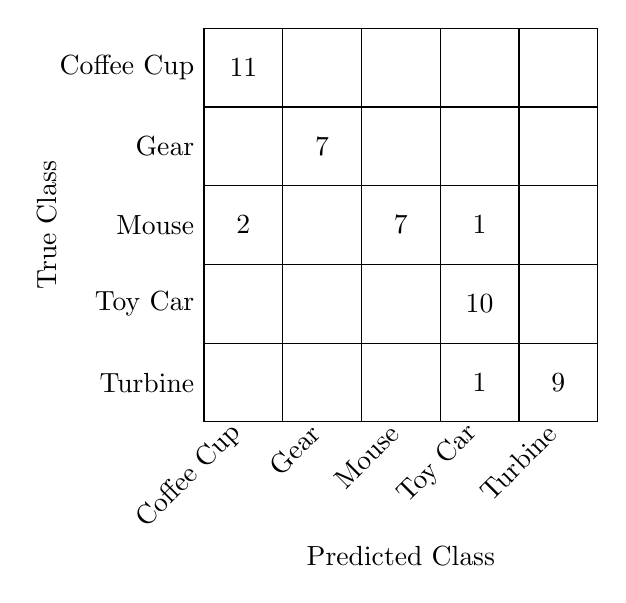
\begin{tikzpicture}

        \foreach \i in {0,...,5} {
          \draw[] (\i,0) -- (\i,5);
          \draw[] (0,\i) -- (5,\i);
        }
      
        \node[anchor=east] at (0,0.5) {Turbine};
        \node[anchor=east] at (0,1.5) {Toy Car};
        \node[anchor=east] at (0,2.5) {Mouse};
        \node[anchor=east] at (0,3.5) {Gear};
        \node[anchor=east] at (0,4.5) {Coffee Cup};
      
        \node[anchor=east, rotate=45] at (0.5,0) {Coffee Cup};
        \node[anchor=east, rotate=45] at (1.5,0) {Gear};
        \node[anchor=east, rotate=45] at (2.5,0) {Mouse};
        \node[anchor=east, rotate=45] at (3.5,0) {Toy Car};
        \node[anchor=east, rotate=45] at (4.5,0) {Turbine};
      
        \node[rotate=90] at (-2,2.5) {True Class};
        \node[] at (2.5,-1.7) {Predicted Class};
      
        \node[] at (0.5,4.5) {11};
        \node[] at (1.5,3.5) {7};
        \node[] at (2.5,2.5) {7};
        \node[] at (3.5,1.5) {10};
        \node[] at (4.5,0.5) {9};
      
        \node[] at (0.5,2.5) {2};
        \node[] at (3.5,0.5) {1};
        \node[] at (3.5,2.5) {1};
      
      \end{tikzpicture}
      }
    } &
    \subfloat[20\%]{
      \resizebox{.45\textwidth}{!}{
      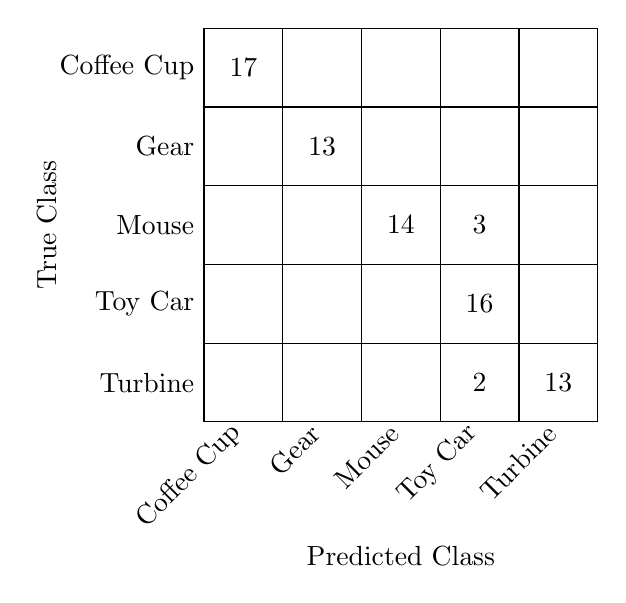
\begin{tikzpicture}

        \foreach \i in {0,...,5} {
          \draw[] (\i,0) -- (\i,5);
          \draw[] (0,\i) -- (5,\i);
        }
      
        \node[anchor=east] at (0,0.5) {Turbine};
        \node[anchor=east] at (0,1.5) {Toy Car};
        \node[anchor=east] at (0,2.5) {Mouse};
        \node[anchor=east] at (0,3.5) {Gear};
        \node[anchor=east] at (0,4.5) {Coffee Cup};
      
        \node[anchor=east, rotate=45] at (0.5,0) {Coffee Cup};
        \node[anchor=east, rotate=45] at (1.5,0) {Gear};
        \node[anchor=east, rotate=45] at (2.5,0) {Mouse};
        \node[anchor=east, rotate=45] at (3.5,0) {Toy Car};
        \node[anchor=east, rotate=45] at (4.5,0) {Turbine};
      
        \node[rotate=90] at (-2,2.5) {True Class};
        \node[] at (2.5,-1.7) {Predicted Class};
      
        \node[] at (0.5,4.5) {17};
        \node[] at (1.5,3.5) {13};
        \node[] at (2.5,2.5) {14};
        \node[] at (3.5,1.5) {16};
        \node[] at (4.5,0.5) {13};
      
        \node[] at (3.5,0.5) {2};
        \node[] at (3.5,2.5) {3};
      
      \end{tikzpicture}
      }
    }
    \\
    \subfloat[50\%]{
      \resizebox{.45\textwidth}{!}{
      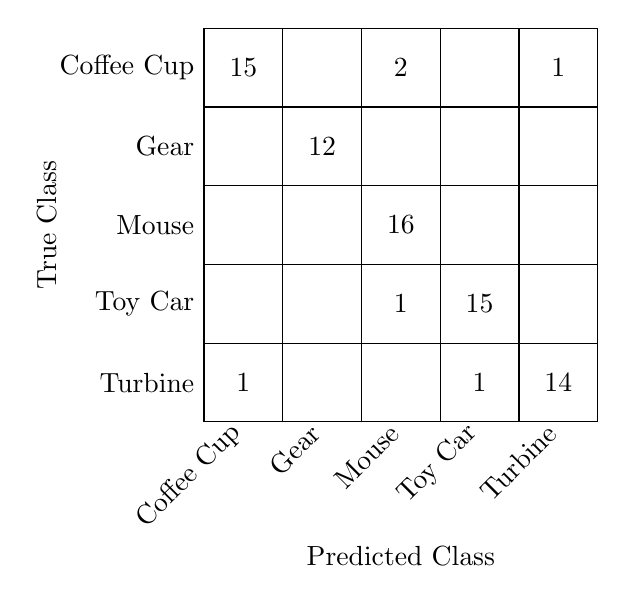
\begin{tikzpicture}

        \foreach \i in {0,...,5} {
          \draw[] (\i,0) -- (\i,5);
          \draw[] (0,\i) -- (5,\i);
        }
      
        \node[anchor=east] at (0,0.5) {Turbine};
        \node[anchor=east] at (0,1.5) {Toy Car};
        \node[anchor=east] at (0,2.5) {Mouse};
        \node[anchor=east] at (0,3.5) {Gear};
        \node[anchor=east] at (0,4.5) {Coffee Cup};
      
        \node[anchor=east, rotate=45] at (0.5,0) {Coffee Cup};
        \node[anchor=east, rotate=45] at (1.5,0) {Gear};
        \node[anchor=east, rotate=45] at (2.5,0) {Mouse};
        \node[anchor=east, rotate=45] at (3.5,0) {Toy Car};
        \node[anchor=east, rotate=45] at (4.5,0) {Turbine};
      
        \node[rotate=90] at (-2,2.5) {True Class};
        \node[] at (2.5,-1.7) {Predicted Class};
      
        \node[] at (0.5,4.5) {15};
        \node[] at (1.5,3.5) {12};
        \node[] at (2.5,2.5) {16};
        \node[] at (3.5,1.5) {15};
        \node[] at (4.5,0.5) {14};
      
        \node[] at (0.5,0.5) {1};
        \node[] at (3.5,0.5) {1};
        \node[] at (2.5,1.5) {1};
        \node[] at (4.5,4.5) {1};
        \node[] at (2.5,4.5) {2};
      
      \end{tikzpicture}
      }
    } &
    \subfloat[80\%]{
      \resizebox{.45\textwidth}{!}{
      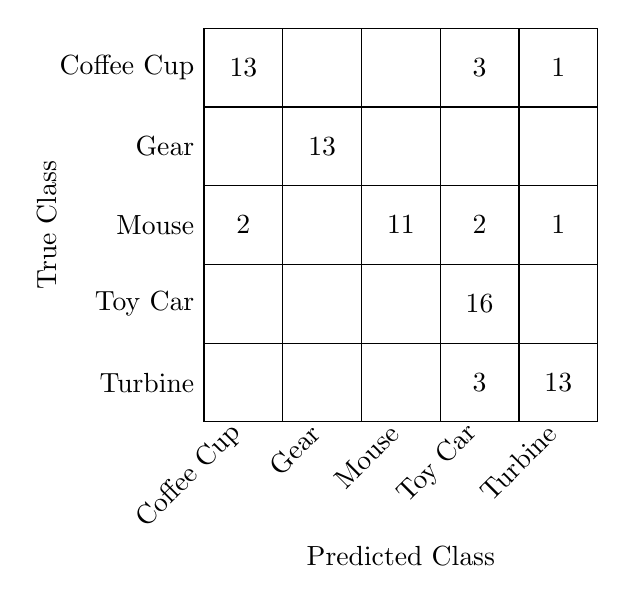
\begin{tikzpicture}

        \foreach \i in {0,...,5} {
          \draw[] (\i,0) -- (\i,5);
          \draw[] (0,\i) -- (5,\i);
        }
      
        \node[anchor=east] at (0,0.5) {Turbine};
        \node[anchor=east] at (0,1.5) {Toy Car};
        \node[anchor=east] at (0,2.5) {Mouse};
        \node[anchor=east] at (0,3.5) {Gear};
        \node[anchor=east] at (0,4.5) {Coffee Cup};
      
        \node[anchor=east, rotate=45] at (0.5,0) {Coffee Cup};
        \node[anchor=east, rotate=45] at (1.5,0) {Gear};
        \node[anchor=east, rotate=45] at (2.5,0) {Mouse};
        \node[anchor=east, rotate=45] at (3.5,0) {Toy Car};
        \node[anchor=east, rotate=45] at (4.5,0) {Turbine};
      
        \node[rotate=90] at (-2,2.5) {True Class};
        \node[] at (2.5,-1.7) {Predicted Class};
      
        \node[] at (0.5,4.5) {13};
        \node[] at (1.5,3.5) {13};
        \node[] at (2.5,2.5) {11};
        \node[] at (3.5,1.5) {16};
        \node[] at (4.5,0.5) {13};
      
        \node[] at (0.5,2.5) {2};
        \node[] at (3.5,0.5) {3};
        \node[] at (3.5,2.5) {2};
        \node[] at (3.5,4.5) {3};
        \node[] at (4.5,2.5) {1};
        \node[] at (4.5,4.5) {1};
      
      \end{tikzpicture}
      }
    }
    \\
  \end{tabular}